\section{A Adoção de Integração, Entrega e Implantação Contínuas nas Empresas}

Como discutido na seção anterior, há evidência sugestiva da adoção de práticas de integração e implantação contínuas (\emph{Continuous Integration} e \emph{Continuous Deployment}) em várias empresas de tecnologia em todo o mundo. Apesar da popularização de CI e CD no desenvolvimento colaborativo de software, ainda há uma grande escassez de estudos que demonstrem como essas práticas foram importadas para a maioria das empresas \cite{empiricalStudy2016}, especialmente as não inseridas entre as empresas globais de desenvolvimento de software.

Uma das tentativas mais recentes de estudo sobre o tema é o desenvolvido por Schermann et al. \cite{empiricalStudy2016}, que busca entender como as práticas geralmente associadas a implantação contínua acharam o seu caminho nas indústrias européia e norte-americana. Nesse estudo os autores utilizaram um método misto de estudo empírico baseado em um pré-estudo na literatura, entrevistas com 20 participantes (pesquisa qualitativa) e um \emph{survey} que recebeu 187 respostas (pesquisa quantitativa). A ideia era questionar até que ponto o conhecimento na área estava dominado por peculiaridades de um pequeno grupo de grandes empresas, como Facebook e Google.

Nesse trabalho, os autores também definem a chamada \emph{stairway to heaven} (escada para o céu, em tradução livre), presente na Figura \ref{stairway}. Ela tem como objetivo definir um caminho de evolução das empresas para um estágio de entregas sofisticado. A escada permeia práticas de integração contínua, implantação contínua e entregas parciais.
Por exemplo, ela sugere que práticas como \emph{trunk based development} --- prática onde todo o código desenvolvido é integrado diretamente no \emph{branch} principal do sistema de controle de versão --- e \emph{full developer awareness} --- prática onde todos os desenvolvedores da equipe estão a par de todos os processos de desenvolvimento e não há concentração de conhecimento em um pequeno grupo ou uma única pessoa --- que aparecem no canto inferior esquerdo da figura deveriam ser adotadas antes de técnicas que aparecem nos níveis mais superiores e a direita na figura, como \emph{dark launches} --- prática onde o código de uma funcionalidade ainda experimental é implantado no ambiente de produção, porém de forma que apenas os desenvolvedores tenham acesso --- que aparece no canto superior direito.

\begin{figure*}
% \begin{center}
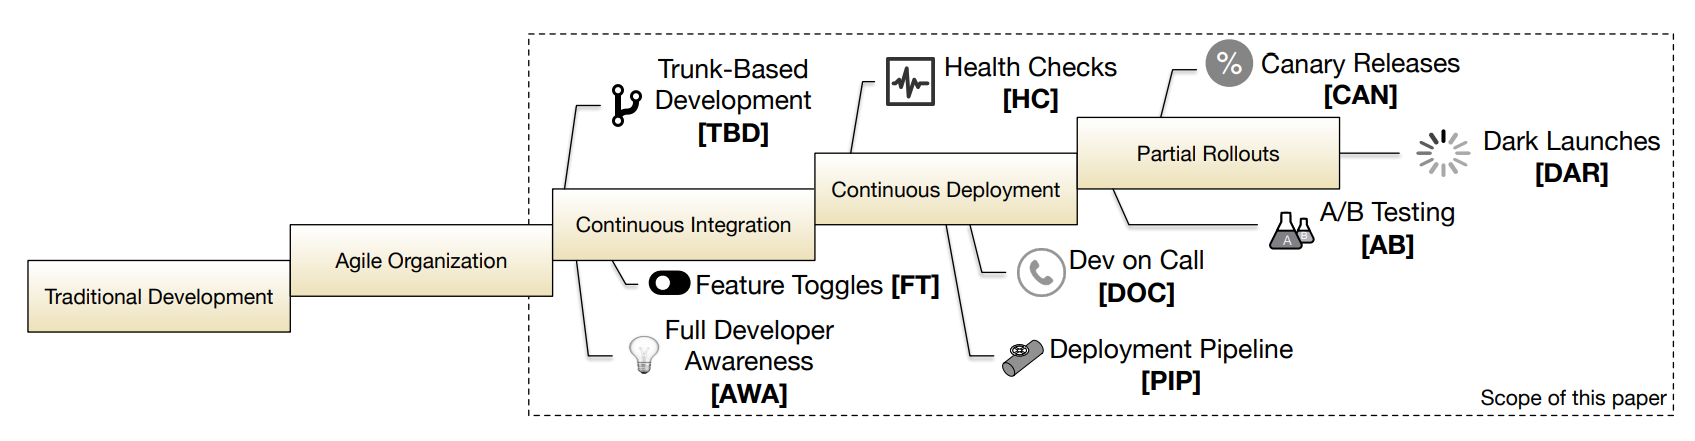
\includegraphics[width=0.75\textwidth]{stairway_to_heaven.png}
% \end{center}
\caption[Stairway to Heaven]{
    A escada de evolução denominada \emph{Stairway to Heaven} \cite{empiricalStudy2016}
}\label{stairway}

\end{figure*}

Através do método misto de estudo os autores descobriram que, no contexto estudado, problemas arquiteturais são geralmente uma das maiores barreiras para a adoção de CD. Não obstante, a técnica de \emph{Feature Toggles} \cite{featureToggles} --- prática que consiste no uso de condicionais ao longo do código para controlar que funcionalidades estarão ativas ou não, possibilitando que funcionalidades ainda não terminadas ou não aprovadas para o ambiente de produção possam ser integradas no código principal sem prejudicar a funcionalidade do sistema  --- como forma de realizar entregas parciais adiciona uma complexidade demasiada e não saudável ao código. Por fim, eles concluem que os desenvolvedores necessitam também de um protocolo baseado em princípios que estabeleçam quando deve-se utilizar técnicas de entregas parciais, por exemplo, que funcionalidades e métricas devem ser testadas por um teste A/B \cite{testsAB} --- prática que consiste em exibir versões diferentes de uma mesma funcionalidade a grupos de usuários distintos, a fim de traçar métricas sobre qual é a mais adequada. Os autores também descobriram que as empresas do estudo não seguem a escada de evolução proposta por eles.

Aprender mais sobre as dificuldades que outras empresas não globais sofrem no processo de adoção de práticas de CI/CD pode gerar mais estudos a respeito de como solucionar tais problemas, assim como mostrar possíveis oportunidades de melhoria e revisão dos processos utilizados. Um trabalho que utilize uma adaptação da metodologia aplicada a uma amostra de um outro contexto pode revelar ainda discrepâncias e semelhanças entre os dois ambientes de estudo. As discrepâncias levantariam pontos de questionamento, pesquisa e até possíveis melhorias aos ambientes envolvidos. Já as semelhanças podem assegurar que as práticas utilizadas já acharam o seu lugar na indústria e funcionam bem assim como a teoria propunha.

Com essa motivação, o presente trabalho procura entender sobre a utilização das práticas de CI/CD nas empresas de Recife para que esses dados sirvam como objeto de pesquisa para levantamento de possíveis dores sentidas pelos desenvolvedores locais que justifiquem a adoção ou não destas práticas. A capital pernambucana é sede de um dos grandes pólos tecnológicos do Brasil:  cerca de 330 empresas e 11 mil trabalhadores, com faturamento anual de R\$ 2,3 bilhões em 2019 \cite{portoDigital}. Um estudo a respeito de como as técnicas de integração e implantação contínua migraram para a indústria de Recife funciona ainda como um \emph{benchmark} de como as empresas estão se portando em relação às novidades presentes na literatura nos últimos anos, assim como levantar possíveis discrepâncias entre empresas situadas na área e as grandes corporações. 

\subsection{Perguntas de pesquisa} 
Com o intuito de entender como as técnicas de integração, entrega e implantação contínua foram importadas para as empresas recifenses, as seguintes perguntas de pesquisa foram formadas:

\vspace{2mm}

\textit{\textbf{PP1}:  Que práticas de CI/CD são utilizadas pelas empresas em Recife?}

\vspace{1mm}

\textit{\textbf{PP2}: O cenário de CI/CD nas empresas em Recife segue o \emph{stairway to heaven} proposto no estudo original?}

\vspace{1mm}

\textit{\textbf{PP3}: Quais são os princípios e práticas subjacentes que governam a adoção de CI/CD na indústria?}

\vspace{2mm}

Para responder as perguntas acima, replicamos parcialmente a pesquisa qualitativa do estudo \cite{empiricalStudy2016} com desenvolvedores recifenses, baseando-se também na mesma lista de definições de cada uma das práticas envolvidas no \emph{Stairway to Heaven}. A pesquisa qualitativa neste contexto foi considerada fundamental para garantir que os entrevistados entendessem claramente as perguntas e excluir possíveis entendimentos errados de termos em inglês, linguagem não nativa de todos os participantes. Além disso, com a pesquisa qualitativa tivemos a oportunidade não só de entender que prática é ou não adotada pela equipe de cada entrevistado, mas também entender o que motivou a adoção, ou o que dificultou ou impediu a adoção. A pesquisa quantitativa realizada pelo estudo original não foi replicada em função da delimitação de escopo deste trabalho, cujo objetivo principal é obter um panorama inicial da adoção de CI/CD nas empresas de Recife, de modo a permitir a o levantamento de indicadores sobre o tema no contexto investigado, que permitam a evolução da pesquisa iniciada com esse estudo.

Além dessas semelhanças e discrepâncias em relação ao estudo original, é importante ressaltar que, as perguntas 1 e 3 são uma adaptação das perguntas 1 e 2 do estudo original \cite{empiricalStudy2016}, respectivamente, incluindo a técnica de integração contínua e restringindo o contexto para Recife. Além disso, uma terceira pergunta foi adicionada (PP2), que foca na escada de evolução proposta pelo artigo. Ela tenta responder se a \emph{stairway to heaven} é seguida no contexto de Recife.
